\section{Discussion} \label{sec:discussion}

\subsection{Iterative Adjustment of Parameters and Environment} \label{subsec:disc_itt}
As briefly described in \cref{subsec:gantt}, the user may evaluate the schedule and robustness analysis results to decide whether or not they accept the schedule as it is, or if they want to adjust the parameters or payloads and test the new configuration. This is a manually process and the user have to decide on which parts of the input that have to be tuned. They are also limited in what the are able to change as it is not possible to modify all of the internal parameters. Some are hidden anyway to lower the required knowledge of the internal tools, UPPAAL \gls{cora} and \gls{smc}, in order to make the system easier to use. 

Instead of having to manually adjust the configuration, it could be possible to make the system self configurable at the end of an iteration. Either to explorer new schedules or a more aggressive robustness analysis. For example, \cref{fig:tool_self_config}  have added an additional step to the tool-chain by allowing the system to loop if the robustness queries were unsatisfied. The system would then have to adjust the variables, such as the [min, max]

\begin{figure}[h]
	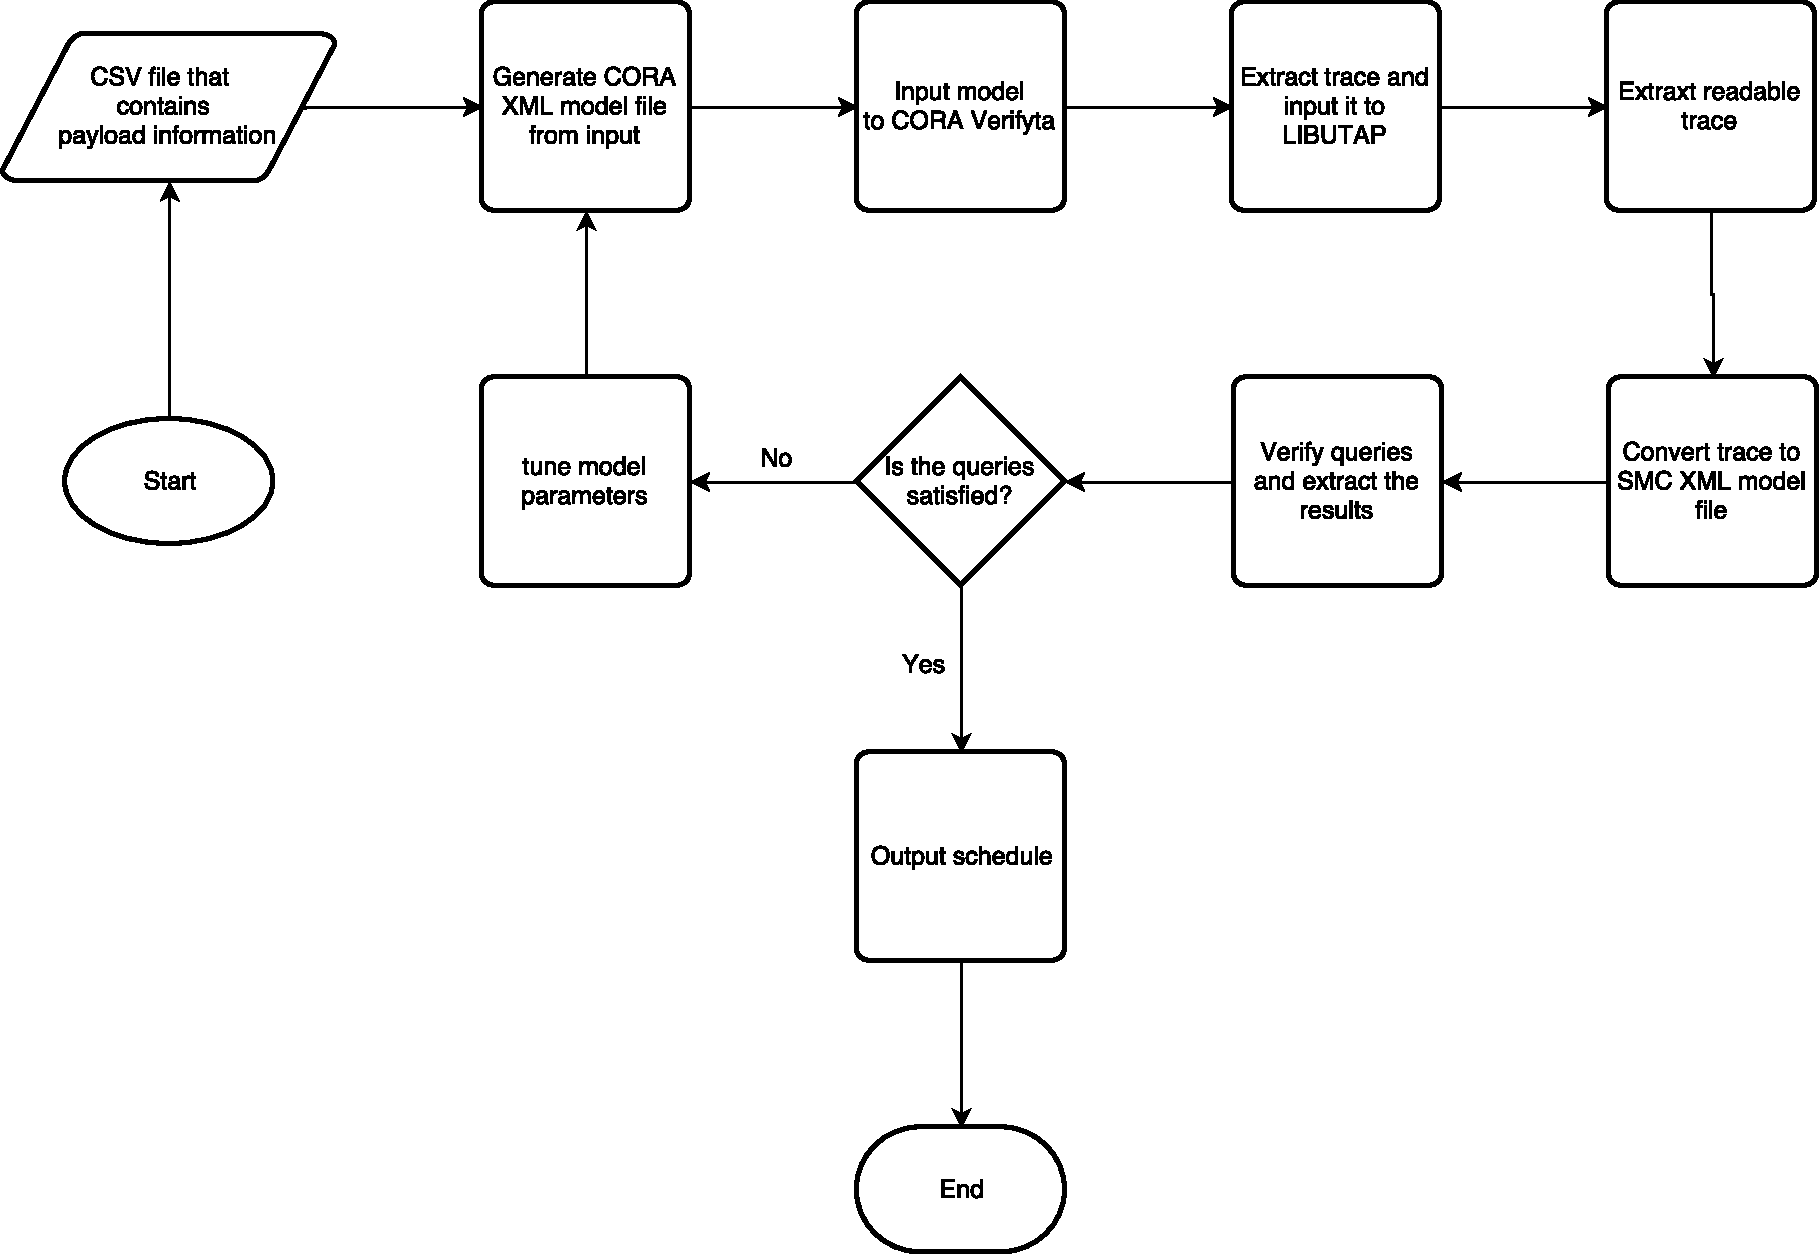
\includegraphics[width=\textwidth]{graphics/tool_chain.pdf}
	\caption{Flowchart that displays the workflow and use of tools}
	\label{fig:tool_self_config}
\end{figure}

problem determine SOC when a battery ends 
logic or in dependencies

Battery Decay


\subsection{Proof of viability}
Vi har kun lavet stikproever
Det tilfldige aspekt goer det besvaergeligt (Random search)